\subsection{2026-09-21 --- Baseline 2: joint multi-output tree}
\label{sec:multioutput}

\subsubsection*{Goal.} Test directly whether the Tokke/Vinje weakness in the baseline
(Section~\ref{sec:baseline}) is a correlated-\emph{output} problem, as hypothesized in
Section~\ref{sec:discussion-next}. Full notebook:
\texttt{src/modeling/multioutput\_tree.ipynb}.

\subsubsection*{Design.} Everything held identical to baseline 1 --- same 54 raw features, same
hyperparameters (\texttt{n\_estimators=200}, \texttt{max\_depth=6}, \texttt{learning\_rate=0.1},
subsample/colsample 0.8), same chronological split (train 2015--2021, validate on held-out
2022), same \texttt{kaggle\_metric.py} scoring --- with exactly one change: a single
\texttt{XGBClassifier} with \texttt{multi\_strategy="multi\_output\_tree"}, trained on all 14
targets jointly, instead of 14 independent single-output models. Each leaf of each tree stores a
vector of 14 probabilities; split choices are optimized jointly across units. This isolates the
independent-vs-joint modeling question specifically, with no other confound.

\subsubsection*{Results.}

\begin{table}[htbp]
  \centering
  \caption{Baseline 1 (independent) vs.\ baseline 2 (joint multi-output tree), 2022 validation.}
  \label{tab:multioutput-auc}
  \resizebox{\linewidth}{!}{%
  \begin{tabular}{lrrr}
    \toprule
    Unit & Baseline 1 (independent models) & Baseline 2 (joint multi-output tree) & $\Delta$ \\
    \midrule
    Tokke\_G3        & 0.528 & 0.656 & +0.129 \\
    Tokke\_G4        & 0.504 & 0.616 & +0.112 \\
    Tokke\_G1        & 0.577 & 0.687 & +0.111 \\
    Vinje\_G1        & 0.519 & 0.622 & +0.102 \\
    Hogga\_G1        & 0.655 & 0.745 & +0.090 \\
    Vinje\_G2        & 0.524 & 0.609 & +0.085 \\
    Vesle\_Kjela\_G1 & 0.724 & 0.773 & +0.049 \\
    Tokke\_G2        & 0.557 & 0.598 & +0.041 \\
    Vinje\_G3        & 0.580 & 0.615 & +0.035 \\
    Byrte\_G1        & 0.751 & 0.784 & +0.033 \\
    Kjela\_G1        & 0.619 & 0.636 & +0.017 \\
    Haukeli\_G1      & 0.564 & 0.554 & $-$0.010 \\
    Lio\_G1          & 0.713 & 0.656 & $-$0.057 \\
    Songa\_G1        & 0.677 & 0.597 & $-$0.080 \\
    \midrule
    \textbf{Overall (micro-average, official metric)} & \textbf{0.647} & \textbf{0.687} & \textbf{+0.040} \\
    \bottomrule
  \end{tabular}%
  }
\end{table}

\begin{figure}[htbp]
  \centering
  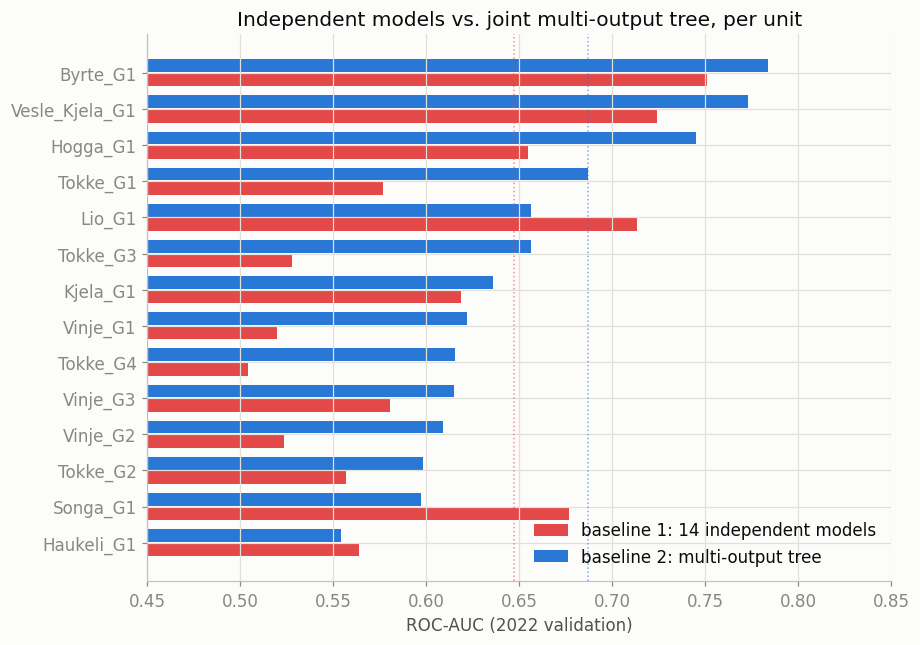
\includegraphics[width=0.85\linewidth]{figures/multioutput_01_per_unit_comparison.png}
  \caption{Per-unit AUC, baseline 1 vs.\ baseline 2, 2022 validation.}
  \label{fig:multioutput-comparison}
\end{figure}

\begin{figure}[htbp]
  \centering
  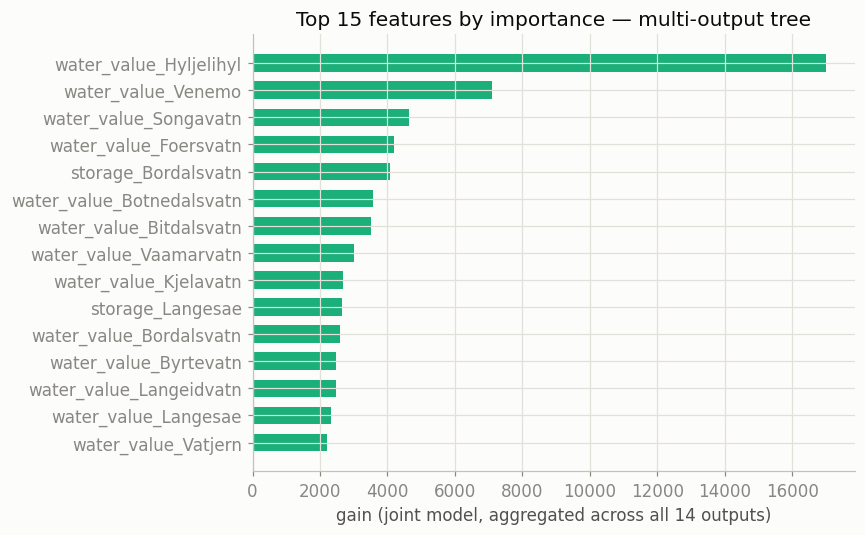
\includegraphics[width=0.75\linewidth]{figures/multioutput_02_feature_importance.png}
  \caption{Top 15 features by gain, joint multi-output model.}
  \label{fig:multioutput-importance}
\end{figure}

\finding{Overall micro-AUC improves from 0.647 to \textbf{0.687} ($+0.040$), and confirms the
hypothesis from Section~\ref{sec:baseline}: the units that improve \emph{most} are almost
exactly the previously-weakest multi-unit-plant units --- all four Tokke units and all three
Vinje units gain $+0.03$ to $+0.13$ AUC, with Hogga\_G1 (topologically adjacent to both, per
Section~\ref{sec:eda}) also improving substantially. Modeling the units jointly does let the
tree exploit the cross-unit correlation that 14 independent models couldn't see.}

\finding{Not a uniform win: \textbf{Songa\_G1 and Lio\_G1 got worse} ($-0.080$ and $-0.057$),
and these were the two best-performing units in baseline 1. Working hypothesis, not yet tested:
the joint model has the same total tree budget (200 trees) shared across all 14 outputs, i.e.\
roughly $14\times$ less dedicated capacity per unit than baseline 1's 200-trees-\emph{each}
setup --- units that didn't need cross-unit information to begin with may simply have lost
modeling capacity to units that did. Worth revisiting (e.g.\ more estimators for the joint
model) before treating this architecture as strictly better.}
\supersededby{sec:capacity}{this capacity hypothesis is tested directly, with a nuanced partial
confirmation.}

This result is tracked in \texttt{report/leaderboard.md} alongside baseline 1.
